\documentclass[12pt]{article}

\usepackage[dvipdfm,%
bookmarks=true,%
bookmarksopen=true,%
bookmarksnumbered=true,%
bookmarkstype=toc,%
pdftitle={CSE 834 Low Pass Filter},%
pdfsubject={},%
pdfauthor={Derek Weitzel, Yutaka Tsutano},%
pdfkeywords={CSCE834, Weitzel, Tsutano, Filter, VLSI}
]{hyperref}

\usepackage{graphicx}
\usepackage{fullpage}

\setlength{\parindent}{0pt}
\setlength{\parskip}{1ex plus 0.5ex minus 0.2ex}

\title{CSE 834 Low Pass Filter}
\author{Derek Weitzel \& Yutaka Tsutano}

\begin{document}
\maketitle

\section{Introduction} \label{sec:introduction}

% Section label inside report.tex
Low pass filters are used in many applications from noise filtering to RF modulation.  Low pass filters are well understood, and include logically simple components: registers, adders, and multipliers.  In this project, we will design a low power low pass filter using the VHDL and the Cadence hardware designer.  We will include optimizations for power such as reducing components and reducing transitions.

In section \ref{sec:design}, we will discuss our design philosophy and design decisions.  In section \ref{sec:implementation} we will describe how we constructed the components and connected them.  Finally, in section \ref{sec:conclusion}, we will discuss problems we experienced in our design and the tools we used.




\section{Design}
\label{sec:design}

\subsection{Q15} \label{sec:q15}

For our filter design, fixed format number format called Q is used. Unlike floating point numbers, Q-format numbers require only standard integer ALU to perform rational number calculations. This means that we do not need to add an FPU to our design which requires additional power.

Q format numbers are represented using the Q notation which is written as Q$m,n$ where $m$ is the number of bits set aside to designate the two's complement integer portion of the number, and $n$ is the number of bits used to designate the fractional portion of the number.

In our case, we use simplified notation Q$n$ since we assume that the numbers are normalized into the range of $[-1, 1)$. Notice that this assumption does not affect the generality of the filter, but it simplifies the multiplication operation because the multiplication result never exceeds the range of $[-1, 1)$.

\begin{figure}[ht]
	\centering
	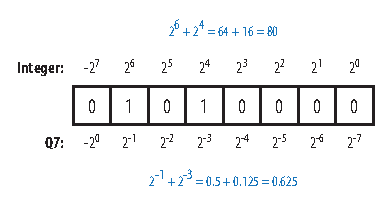
\includegraphics[scale=1.5]{images/q7}
	\caption{Comparison between integer and Q7 format.}
	\label{fig:q7}
\end{figure}

Figure \ref{fig:q7} shows the comparison between two's complement integer and Q7 numbers. The only difference between the two is the weight assigned for each bit.

\subsection{Filter Characteristics}

\begin{figure}[ht]
	\centering
	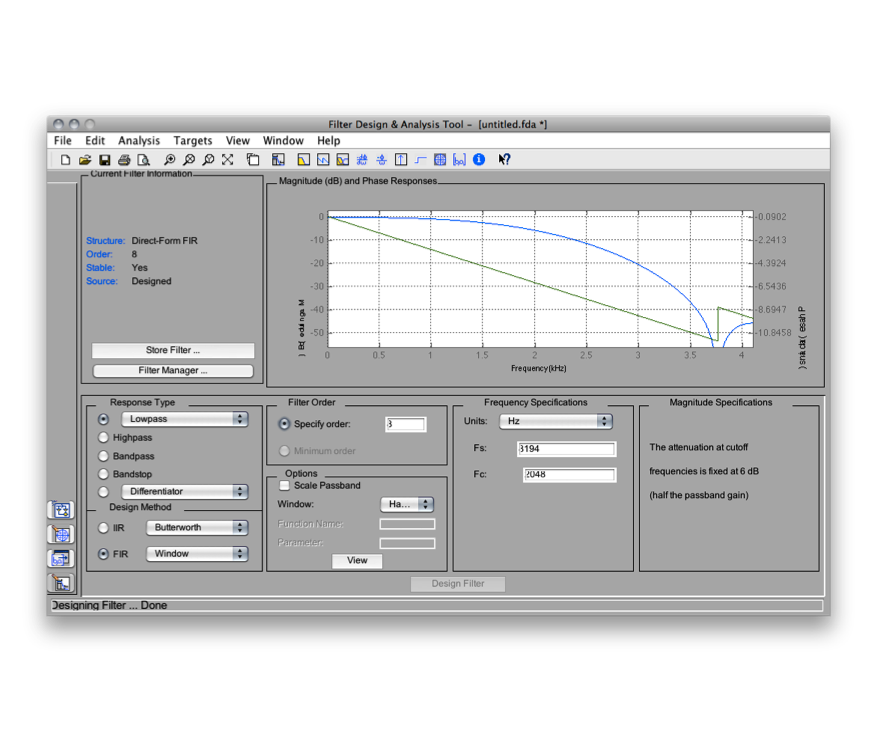
\includegraphics[scale=1]{images/matlab}
	\caption{Matlab.}
	\label{fig:matlab}
\end{figure}

\subsection{Input \& Output}
The input and output of our design are shown in table \ref{table:inputoutput}

\begin{table}[ht]
\centering
\begin{tabular}{l | l | c}
\hline
Input/Output & Description & Bits \\
\hline \hline
Input & Clock & 1 \\
Input & Data In & 16 \\
Output & Convolution & 16 \\
\end{tabular}
\caption{Description of input and output to the filter}
\label{table:inputoutput}
\end{table}



\subsection{Power Optimization}

We will tackle power concerns by optimizing the tree of adders (see Figure \ref{fig:diagram}).  Since we have a constant number of adders, we can create a large adder that will be able to minimize redundant gates.  Further, because of the symmetric property of the filter, we can minimize the number of multipliers by adding symmetric registers, then multiplying by the coefficient.  





\section{Implementation} \label{sec:implementation}
\subsection{VHDL Design}


\subsection{Functional Verification}



\subsection{Synthesis}



\subsection{Final Layout \& Routing}


\section{Conclusion} \label{sec:conclusion}

% Conclusion

In this project, we created a power optimized low pass filter.  We avoid using a floating point unit by utilizing the Q15 format.  The filter is symmetric, allowing for optimizations.  The input and output is kept simple.    The power optimizations where done at design time using the algorithmic level.  The components where developed in VHDL.  The design was verified both at the functional level with a C++ program, and using the VHDL through a simulator.  The components where synthesized using the Cadence tools.  Finally, the layout was done using the autorouter in Cadence.

Both the DRC and LVS for the final layout failed.  During autorouting, the router introduced DRC errors.  LVS fails due to a cadence configuration error that I was unable to correct.  Although both DRC and LVS fail, the VHDL simulates correctly and is functionally correct.  



\if 0

\section{Overview}
In this project, we will create a 16 bit low pass filter.  This filter is similar to those used in audio processing.  This specific properties of the filter where picked to simplify the design.

For each clock period, the circuit will:
\begin{itemize}
\item Shift the registers.  This will pop the last register's value, and save the data\_in value to the first register.
\item Calculate the convolution of the values inside the 8 registers.
\end{itemize}

The coefficients are fixed, therefore they will be constant in the multipliers, simplifying the design.  The input will be 1 bit for the clock, and 16 bits of input data.  The output will be the 16 bit output.  The format of the input and output will be Q15.  The multipliers  and registers will be done in VHDL in order to simplify design.

\begin{table}[ht]
\centering
\begin{tabular}{l | l | c}
\hline
Input/Output & Description & Bits \\
\hline \hline
Input & Clock & 1 \\
Input & Data In & 16 \\
Output & Convolution & 16 \\
\end{tabular}
\end{table}

We will tackle power concerns by optimizing the tree of adders (see Figure \ref{fig:diagram}).  Since we have a constant number of adders, we can create a large adder that will be able to minimize redundant gates.  Further, because of the symmetric property of the filter, we can minimize the number of multipliers by adding symmetric registers, then multiplying by the coefficient.  

\section{Timeline}

11/2 - 11/8: Registers and Multipliers \\
11/8 - 11/23: Optimized Adder \\
11/23 - 12/2: Report - Finalizations \\

\section{Filter Properties}
These are the specific filter properties that where used to calculate the Coefficients seen in Table \ref{tab:coefficients}.

Sampling Frequency Fs = 8194 Hz \\
Cut-off Frequency = 2048 Hz \\
FIR (Lowpass Filter with Hamming Window) \\

\begin{table}[ht]
\centering
\begin{tabular}{ c | r }
\hline
Coeffiecient & Value \\
\hline \hline
$C_0$ & -1.55107884796477e-18 \\
$C_1$ & -0.022663985459552 \\
$C_2$ & 1.04697822237622e-17 \\
$C_3$ & 0.273977082565524 \\
$C_4$ & 0.497373805788057 \\
$C_5$ & 0.273977082565524 \\
$C_6$ & 1.04697822237622e-17 \\
$C_7$ & -0.0226639854595526 \\
$C_8$ & -1.55107884796477e-18 \\
\end{tabular}
\caption{Coefficient values}
\label{tab:coefficients}
\end{table}


%\begin{figure}[ht]
%\centering
%\includegraphics[scale=0.55]{../coeffs.png}
%\caption{Plot of coefficients.  Notice the symmetry.}
%\label{fig:plotcoefficients}
%\end{figure}

%\begin{figure}[ht]
%\centering
%\includegraphics[scale=0.55]{../filter_design.png}
%\caption{Plot of filter characteristics}
%\label{fig:characteristics}
%\end{figure}

%\begin{figure}[ht]
%\centering
%\includegraphics[scale=0.55]{../Diagram.png}
%\caption{Logical diagram of the data flow.}
%\label{fig:diagram}
%\end{figure}

\fi

\end{document}
